\section{A visit to the Southern Reaches via Stuck in Paradise}

\subsection{Overview} 
Cavers undertaking a trip to Atlantis and beyond will visit one of the only locations where stalactites are found in Sistem Migovec. As well as long and arduous horizontal passages, the trip involves a memorable muddy pitch, a large chamber with interesting sediment and the chance to witness biological remains of trogloxenes.

\subsection{Friendship Gallery to Hidden Surprise}
From Camp X-ray, it is necessary to go along Friendship Gallery back to the bottom of Zimmer Pitch and ascend the rope to the Cheetah window, climbing into the cleft several rebelays until the passage levels off and slopes towards a pitch head. A careful descent of the Cheetah pitch lands on a ledge, 5m from the boulder strewn floor proper. The way to Hidden Surprise is on the right hand opening, up into a large trunk passage. A muddy descent leads to a small, roped drop onto a perpendicular, but still large passageway. On the far side, a hidden squeeze through boulders (paper note towards Red Baron) leads to a short crawl over loose blades of rock to the next pitch.
\subsection{Hidden Surprise to Red Baron traverse}
At the bottom, the way on is again through boulders, and slightly up to the \emph{Milka Pitch}: a rope on the right handside leads to a tight rebelay and a traverse to the right before a final section of descent on the opposite wall, which lands on a pile of boulders. A short, roped drop through boulders and a wriggle leads to the key breakthrough of \emph{Kamikaze}. 

\textit{At the PSS, the upwind continuation eventually leads to \emph{Kamikaze} and the \emph{A Pun too Far} streamway}. 

Downwind ends at a boulder collapse  Red Baron chamber, sloping towards the right to a pit. The namesake traverse goes over the pit.

\subsection{Red Baron traverse to Stuck in Paradise}
On the other side of the traverse, an ascending boulder strewn tunnel, the \emph{Throne Room} enlarges at a pitch. It is necessary to climb past one rebelay and carry on climbing on another rope to reach \emph{Amazing Grace}, another trunk route. The way goes past some larger collapse chambers before a marked up junction where one climbs down to a boulder choke. Following the draught through the boulders and keeping high and left in the following, sloping chamber, one eventually emerges into the start of \emph{Puff the Magic Dragon}, the continuation of the trunk route. Past two handline climbs down, the passage terminates at the start of \emph{Stuck in Paradise} pitch.

\begin{figure*}[t!]
\checkoddpage \ifoddpage \forcerectofloat \else \forceversofloat \fi
\centering
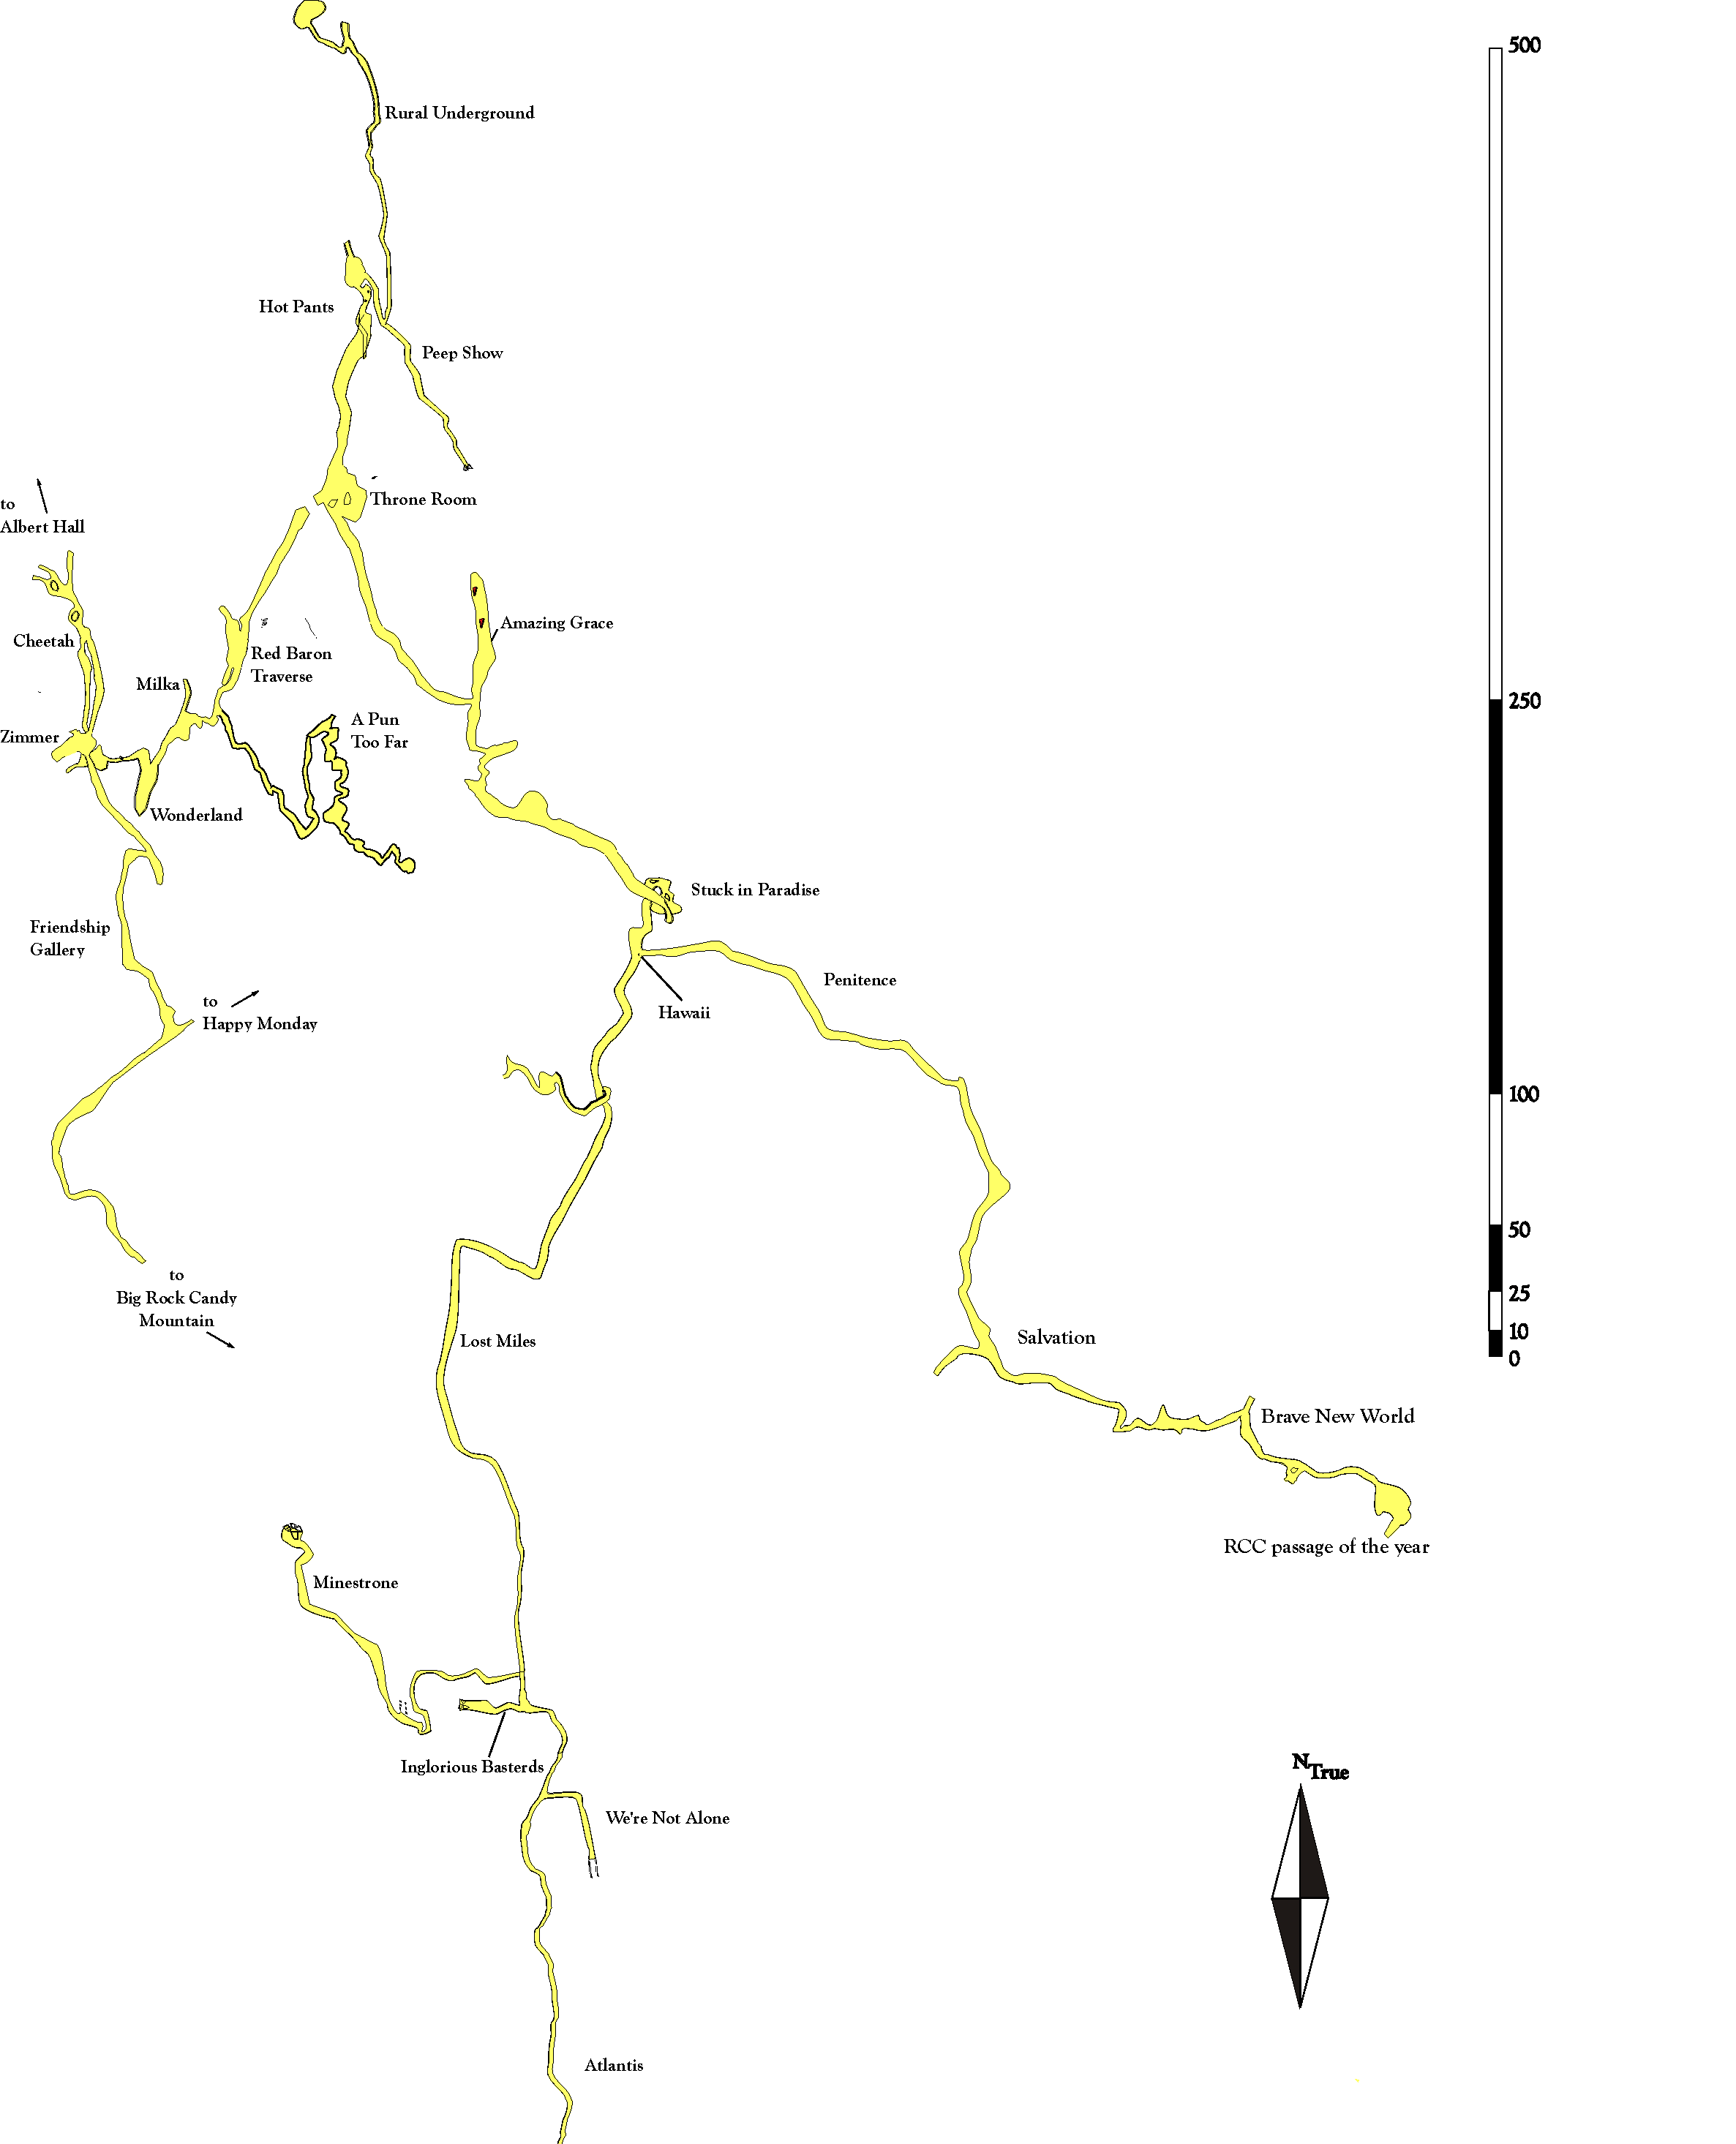
\includegraphics[width=\textwidth]{PDF_maps/Paradise.pdf}
\caption{Plan view of the lower passages off Cheetah pitch}
\label{paradise}
\end{figure*}

\subsection{Stuck in Paradise to Sic Semper Tyrannis}
Beginning with a short climb up and traverse to reach better rock, the route then spirals down one of the shafts of the pitch, which is broken in several sections. Finally, a constriction through boulders leads to the final deviated rope and a landing at Hawaii junction, where a daren drum full of collected drips offers the only available water between \emph{Zimmer} and \emph{Brezno Slapov}. What follows is a low ceiling, but mainly walking passage heading south, interrupted by a short perpendicular climb where wall crystals are particularly prominent. Farther on, the passage heads south again, lowering to a hands and knees crawl to a boulder choke. A short wriggle leads to the start of \emph{Atlantis}, which is the continuation of the abandoned phreatic tube. 600m of varied crawling to walking passage, hosting many decorations  where the way on is always south, past the Minestrone and We're Not Alone junctions. Towards then end, the passage slopes down to a boulder junction where the sound a waterfall from Brezno Slapov can be heard. 

\subsection{Sic Semper Tyrannis to First Draft}
A the junction, the start of Sic Semper Tyrannis is a squeeze over a flat boulder to a cobble-floored alcove and and the start of a multilevel rift. Bearing left, a couple of traverses over pits leads to a T junction. 

\textit{Right leads to the start of \emph{Pleasure Palace}, via a 10m pitch, which eventually reconnects to the \emph{Meridian Way} via a 300m crawl. Beyond the pitch lies a boulder chamber with several ways on, including a climb to \emph{Helm's Deep} chamber or down to the streamway and \emph{Davy Jones Locker}. The water eventually cascades down to the \emph{Lethe} streamway.}

Left is the way on, up into a multilevel rift heading south, Jericho. A short climb can be bypassed by a narrow squeeze, which lead on to a further ascent and descent into Squidgy Goodness. The remnants of a dormouse can be found at the bottom of small 2m climb down. Further on, Jetstream, so named because of the chilling strong draught takes the shape of rift with wide ledges where it is necessary to climb up to a muddy squeeze and slope down to a boulder choke. Past the boulders is the start of \emph{Final Draft}.

\subsection{Final Draft to Choke-a-Bloke}
At the next junction, turning left past some decorated alcoves and crawling through white sand pools quickly leads to the start of a slanting pitch. 25m below, the pitch enlarges as it meets an abandoned phreatic passage. North connects to the \emph{Pleasure Palace}. South is the \emph{Meridian Way}, 150m of easy walking passage past some dormouse excrement, hair and bones to a boulder choke. The passage continues beyond to a junction. The obvious continuation drops down to the south west, ending after 100m at a boulder choke and an unclimbed aven (\emph{Empty Quarter}). Back at the junction, a too tight squeeze marks the end of \emph{Choke-a-Bloke} and the end of this trip, not 350m away from mountain side whence the rodents came to die.



\begin{figure*}[t!]
\checkoddpage \ifoddpage \forcerectofloat \else \forceversofloat \fi
\centering
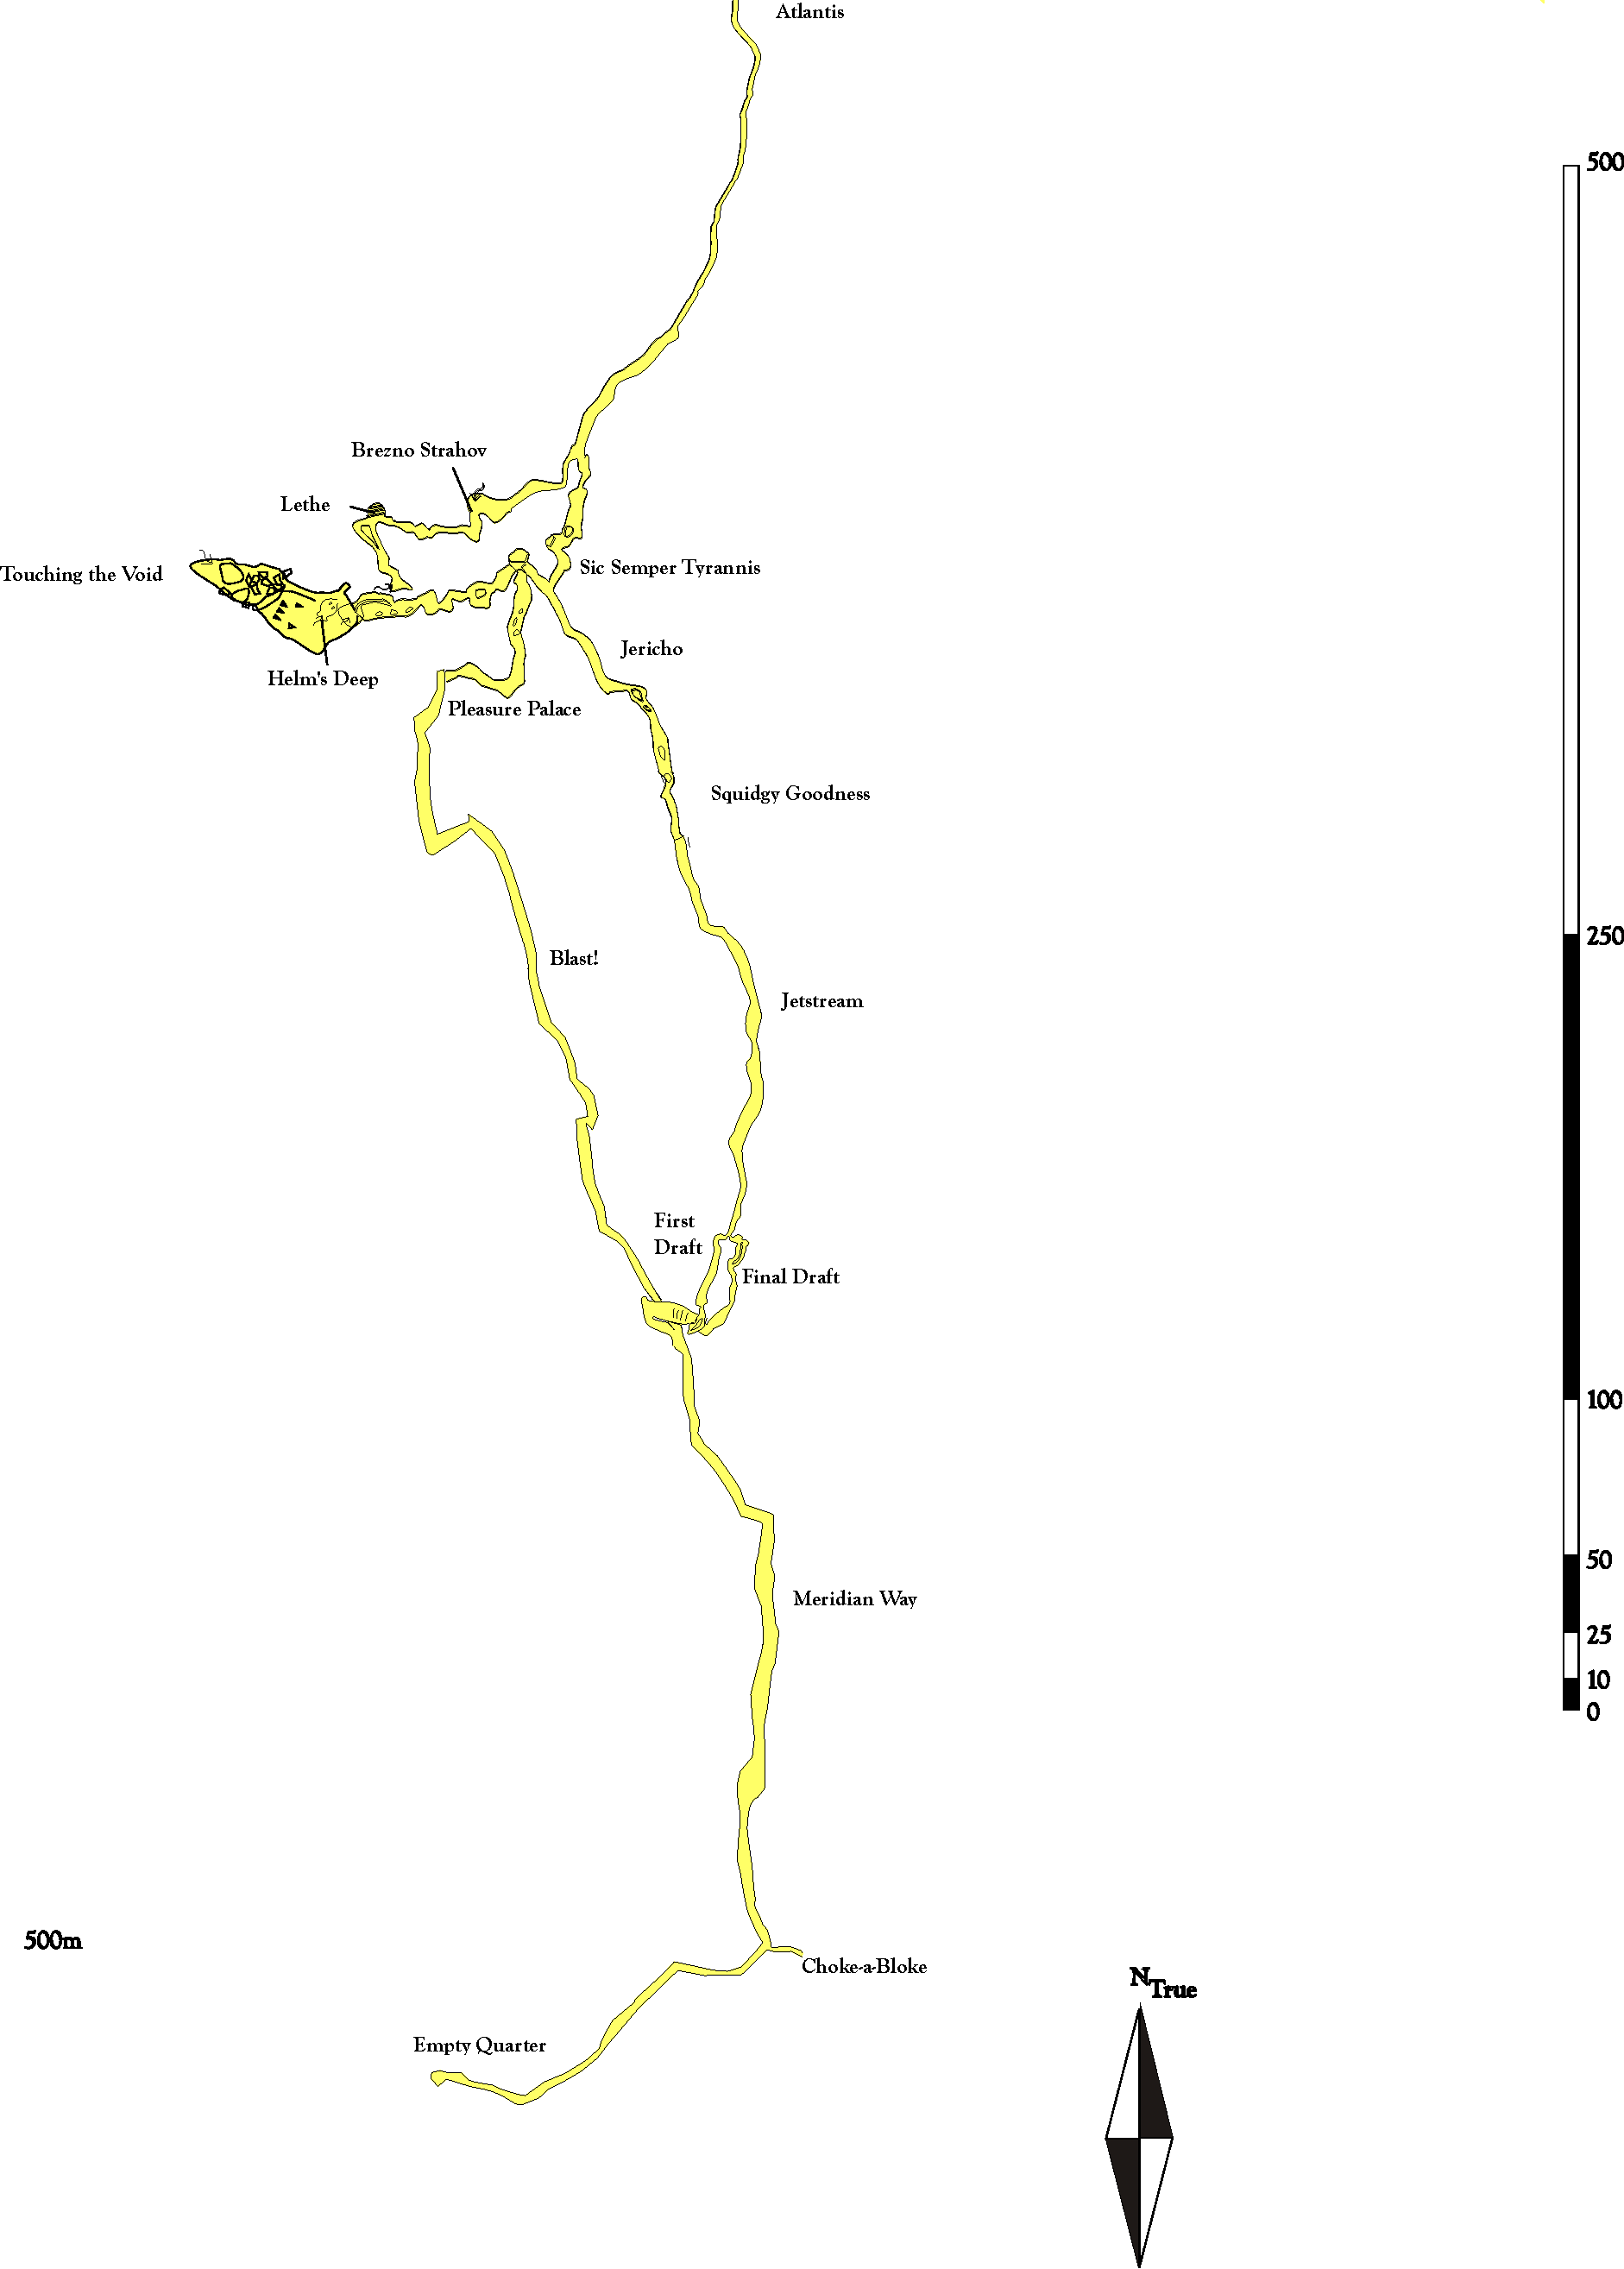
\includegraphics[width=\textwidth]{PDF_maps/Paradisesouth.pdf}
\caption{Plan view of the lower passages off Cheetah pitch}
\label{paradise}
\end{figure*}